\documentclass{article}
\usepackage{fullpage}
\usepackage[czech]{babel}
\usepackage{amsfonts}
\usepackage{amsmath}
\usepackage{graphicx}
\usepackage{caption}
\graphicspath{{images/}}

\title{\vspace{-2cm}Fyzika druháku\vspace{-1.7cm}}
\date{}
\author{}

\begin{document}
\maketitle

\part{Deformace}

  \begin{minipage}{0.25\textwidth}\raggedleft
    \begin{itemize}
      \item typy:
      \begin{itemize}
        \item tahem/tlakem
        \item kroucením
        \item ohybem
        \item smykem
      \end{itemize}
    \end{itemize}
  \end{minipage}
  \hspace{0.5cm}
  \noindent\begin{minipage}{0.12\textwidth}
    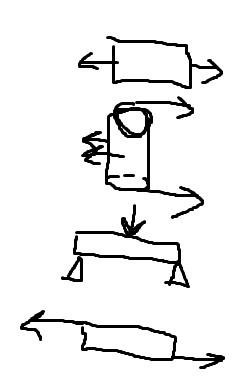
\includegraphics[width=0.9\linewidth]{deformace}
  \end{minipage}

  \section{Deformace tahem/tlakem}

    \begin{itemize}
      \item Normálové nápětí:
      	\begin{equation*}
          \sigma=F/S; \ [N/m^2] = [Pa]
        \end{equation*}
        \begin{center}
          \vspace{-0.25cm}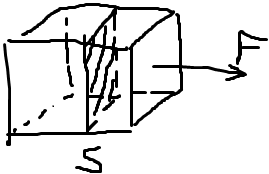
\includegraphics[width=0.12\textwidth]{normalove_napeti}\vspace{-0.25cm}
        \end{center}
      \item Změna délky:
        \begin{equation*}
          \Delta l = l - l_0; \ [m]
        \end{equation*}
      užitečnější většinou relativní prodloužení:
        \begin{equation*}
          \varepsilon = \Delta l/l_0; \ [bezrozm.]
        \end{equation*}
    \end{itemize}

    \subsection{Deformační křivka}
      \begin{center}
        \vspace{-0.1cm}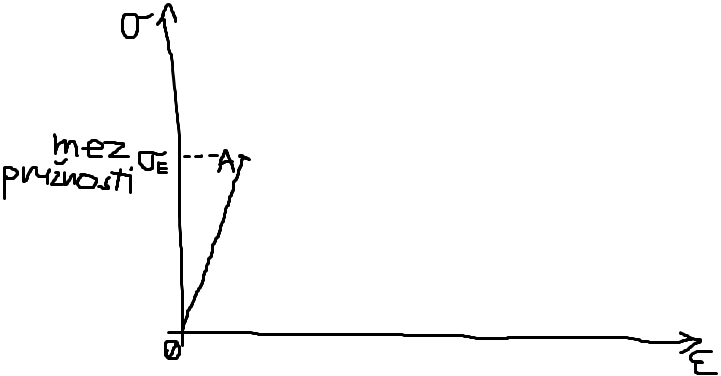
\includegraphics[width=0.75\linewidth]{deformacni_krivka}\vspace{-0.25cm}
      \end{center}

      \begin{itemize}
        \item lineární úsek (0 - A)
        \begin{itemize}
          \item pružná deformace
          \item vratná
          \item platí Hookův zákon:
            \begin{equation*}
              \varepsilon \propto \sigma
            \end{equation*}
          tedy slovy: relativní prodloužení je přímo úměrné napětí (ano, to je symbol pro přímou úměrnost, zapamatujte si ho)
            \begin{equation*}
              \sigma = E*\varepsilon
            \end{equation*}
          E - Youngův modul pružnosti (např. ocel = 220 GPa, cín = 55 GPa, tj. tlak potřebný, abychom objekt roztáhli na dvojnásobnou délku)
        \end{itemize}
        \item nelineární deformace (A - B)
        \begin{itemize}
          \item plastická deformace
          \item protažení bylo dost velké, aby přesunulo atomy v krystalické mřížce na jiné místo
          \item materiál tedy ztráci schopnost se po deformaci vrátit do původního tvaru
          \item při překročení meze pevnosti se materiál prostě trhá na dva kusy
        \end{itemize}
      \end{itemize}

        \subsubsection{Příklady}
        \begin{enumerate}
          \item O kolik se protáhne ocelový drát když na něj zavěsíme závaží:
          \begin{equation*}
            d = 1 mm;
            l = 5 m;
            m = 30 kg;
            E = 220 GPa
          \end{equation*}
          \begin{itemize}
            \item[]
          \end{itemize}
          \begin{equation*}
            \sigma=\frac{F}{S}=\frac{300}{\pi*0,0005^2}
          \end{equation*}
          \begin{equation*}
            \varepsilon = \frac{\sigma}{E}
          \end{equation*}
          \begin{equation*}
            \varepsilon = \frac{F}{S*E}=\frac{\Delta l}{l_0}
          \end{equation*}
          \begin{equation*}
            \Delta l = \frac{F*l*0}{S*E}=8,7*10^{-3} m = 8,7 mm
          \end{equation*}
          \item Na ocelové lanko zavěsíme závaží. Jak těžké může být, aby se lanko nepřetrhlo:
          \begin{equation*}
            d = 1 mm;
            \sigma_p = 1,3 GPa;
            K = 5
          \end{equation*}
          \begin{enumerate}
            \item závaží je v klidu
            \item závaží se hýbe nahoru
            \begin{equation*}
              a = 1 m/s^2
            \end{equation*}
            \item jako kyvadlo OBRAZEKOBRAZEK
          \end{enumerate}
        \end{enumerate}

\end{document}
